\documentclass{article}
\usepackage{tikz} 
\usepackage[utf8]{inputenc}
\usepackage{amsmath}
\usepackage{listings}
\usepackage{amsfonts}
\usepackage{amssymb}
\usepackage{tabularx}
\usepackage{enumitem}
\usepackage{algorithm}% http://ctan.org/pkg/algorithm
\usepackage[noend]{algpseudocode}% http://ctan.org/pkg/algorithmicx
\usepackage{tikz}
\usepackage{graphicx}


\usepackage{subcaption}
\usepackage{multicol,caption}
\usepackage{geometry}
 \geometry{
 a4paper,
 total={210mm,297mm},
 left=20mm,
 right=20mm,
 top=20mm,
 bottom=20mm,
 }

\usetikzlibrary{arrows,positioning,shapes,fit} 
\pgfarrowsdeclarecombine{ring}{ring}{}{}{o}{o}
\thispagestyle{empty}
\DeclareMathOperator{\ringarrow}{\raisebox{0.5ex}{\tikz[baseline]{\draw[ring->](0,0)--(2em,0);}}}

\definecolor{talk}{HTML}{729FCF}
\definecolor{talk2}{HTML}{E8A753}
\definecolor{grey}{HTML}{DBDCDD}
\renewcommand{\vec}[1]{\boldsymbol{#1}}
\tikzset{
    %Define standard arrow tip
    >=stealth',
    %Define style for boxes
    observed/.style={
   	circle,
   	rounded corners,
   	draw=black, thick,
   	minimum width=2.3em,
   	minimum height=2.3em,
   	font=\footnotesize,
   	text centered,
   	fill=talk!50
   },
   latent/.style={
   	circle,
   	rounded corners,
   	draw=black, thick, dashed,
   	minimum width=2.2em,
   	minimum height=2.2em,
   	font=\footnotesize,
   	text centered
   },
    % Define arrow style
    pil/.style={
           o->,
           thick,
           shorten <=2pt,
           shorten >=2pt,},
    sh/.style={ shade, shading=axis, left color=red, right color=green,
    shading angle=45 },
observedrect/.style={
	rectangle,
	rounded corners,
	draw=black, thick,
	minimum width=3em,
	minimum height=1.5em,
	font=\footnotesize,
	text centered,
	fill=talk2!80
},  
 target/.style={
	circle,
	rounded corners,
	draw=black, thick,
	minimum width=2.3em,
	minimum height=2.3em,
	font=\footnotesize,
	text centered,
	fill=talk2!80
},
empty/.style={
	circle,
	rounded corners,
	minimum width=.5em,
	minimum height=.5em,
	font=\footnotesize,
	text centered,
},
}
   
\begin{document}
%\pagestyle{empty}

 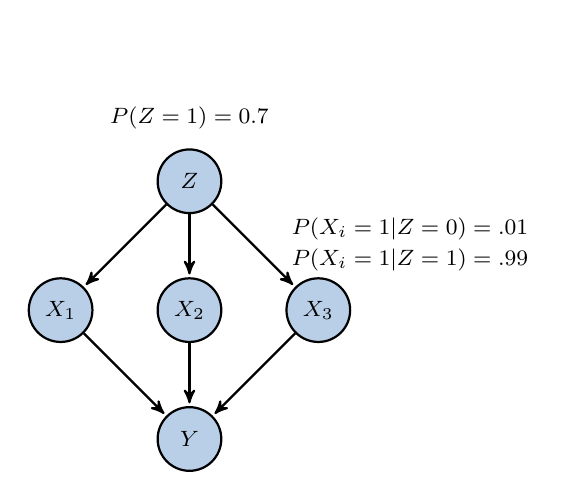
\begin{tikzpicture}[->,>=stealth',shorten >=1pt,auto,node distance=.8cm,
thick,main node/.style={observed}, em/.style={empty},background rectangle/.style={fill=olive!45}]
%every node/.style={scale=0.6}
%nodes
\node[main node](1){$X_{1}$};
\node[main node, right=of 1](2){$X_{2}$};
\node[main node, above=of 2](6){$Z$};
\node[em, above of=6](7){$P(Z=1)=0.7$};
\node[em, right of=6,xshift=2cm,yshift=-1cm](8){$P(X_i=1|Z = 1)=.99$};
\node[em, above of=8,yshift=-.4cm](9){$P(X_i=1|Z = 0)=.01$};
\node[main node, right=of 2](3){$X_{3}$};
\node[main node, below =of 2](5){$Y$};
\path[every node/.style={font=\tiny}]
(1) edge (5)
(2) edge (5)
(3) edge (5)
(6) edge (1) edge (2) edge (3);
\end{tikzpicture} 

\end{document}